Casos de uso todas las funciones del engine y diseñarlo para que la infra sea a través de consola de comandos (preparando para que luego debido a la comunicación rpc devolver los datos sea muy complicado si lo dividimos en otro comando y decidimos absorver este dominio)

El sistema está pensado para que el programa a ejecutar sea de libre decisión del cliente. pero vamos a aprovechar la oportunidad para crear un programa de control y profundizar tanto en el uso del lenguaje como en los conocimientos relacionados con este master. En concreto el control automático. Uno do los programas que podrá ejecutar será un control PID.



\begin{figure}[H]
    \centering
    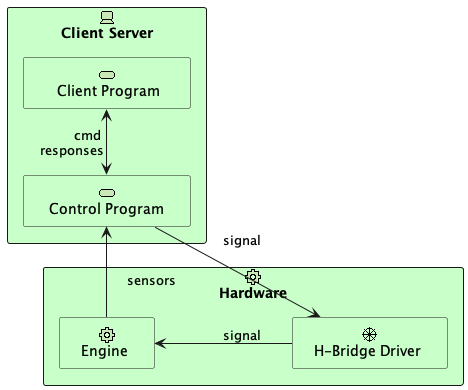
\includegraphics[height=0.3\textheight]{./part/Proyecto_ejecutivo/memoria_descriptiva/descripcionDelProyecto/control/uml/controlConcept}
    \caption[Diagrama componentes]{}\label{fig:controlConcept}
\end{figure}

\subparagraph{Dominio}

\begin{figure}[H]
    \centering
    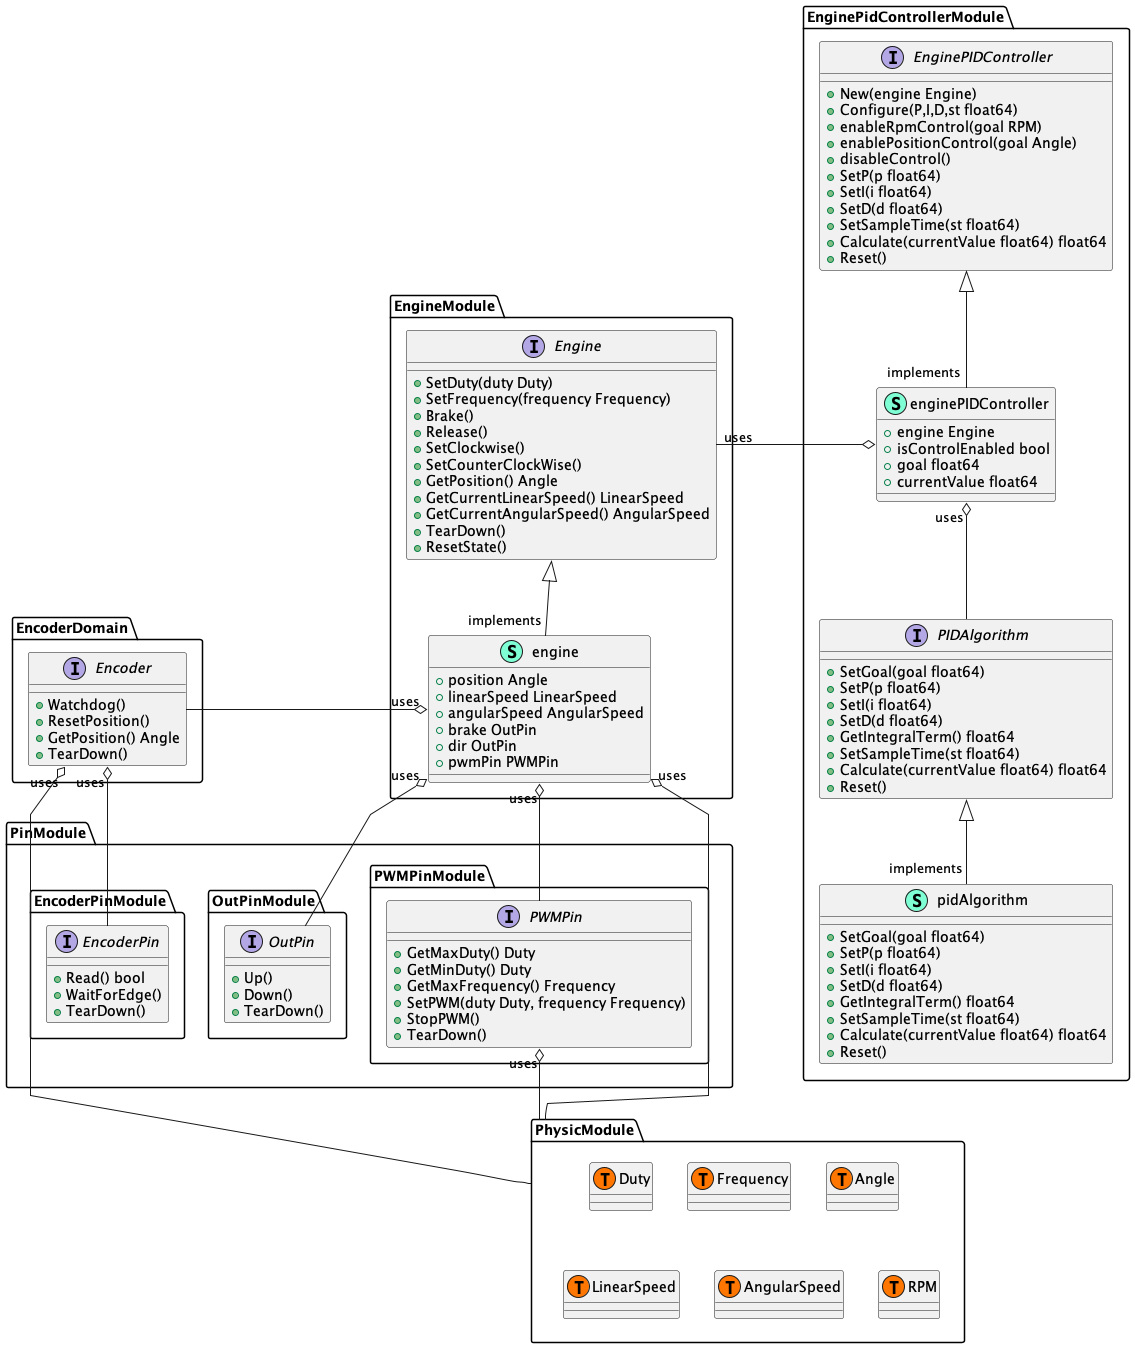
\includegraphics[height=0.4\textheight]{./part/Proyecto_ejecutivo/memoria_descriptiva/descripcionDelProyecto/control/uml/controlDomain}
    \caption[Diagrama de objetos de dominio]{}\label{fig:controlDomain}
\end{figure}

\begin{itemize}
    \item StepDomain
\end{itemize}

\subparagraph{casos de uso}

Vamos a describir los casos de uso que podrán ejecutarse en el programa manager. Tenemos 2 Entities y dos aggregate root.

\begin{itemize}
    \item Step
    \item Result
\end{itemize}

\textbf{ejecutar Step}

\subparagraph{estructura de carpetas}

En el proyecto constará de 4 carpetas principales

\tiny
\dirtree{%
    .1 Project .
        .2 Domain.
        .2 Application.
        .2 Adapter.
        .2 Bootstrap.
}
\normalsize

\textbf{Dominio}

\begin{figure}[H]
    \tiny
\dirtree{%
    .1 Domain.
        .2 Step.
            .3 StepVo.
            .3 Repository.
                .4 consoleWrite.
            .3 Services.
                .4 Executor.
        .2 Result.
            .3 ResultVo.
}
\normalsize
    \caption[Diagrama de objetos de dominio]{}\label{fig:1-controlDomain}
\end{figure}

\textbf{Aplicación}

\tiny
\dirtree{%
.1 Application.
    .2 Port.
        .3 in.
            .4 Step.
                .5 Execute.
                    .6 Command.
                    .6 UseCase.
}
\normalsize

\textbf{Adapters}

\tiny
\dirtree{%
    .1 Adapter.
        .2 in.
            .3 GRPC.
                .4 Harán uso de los useCases de aplicación cuando llegue una request RPC.
            .3 Console.
                .4 Por ejemplo si quisieramos ejecutar los casos de uso mediante terminal.
        .2 out.
            .3 console.
                .4 implementación de los repository de llamada a los servidores clientes.
}
\normalsize





